\documentclass[runningheads]{llncs}
\usepackage{graphicx}
\usepackage{url}
\usepackage{cite}
\usepackage{amsmath}
\usepackage[colorlinks=true, linkcolor=blue, urlcolor=blue]{hyperref}

\begin{document}

\title{Comparación de Sistemas de Recuperación de Información: BM25 vs. DPR}
\titlerunning{Comparación de Sistemas de Recuperación de Información}
\author{Eisler Francisco Valles Rodriguez \and Rafael Acosta Márquez \and Jorge Alejandro Pichardo}
\authorrunning{Comparación de Sistemas de Recuperación de Información: BM25 vs. DPR}
\institute{Universida de La Habana, La Habana, Cuba}

\maketitle

\begin{abstract}
Este informe presenta una comparación entre dos sistemas de recuperación de información: BM25, un modelo tradicional sin el uso de inteligencia artificial, y Dense Passage Retrieval (DPR), un modelo moderno que integra técnicas de inteligencia artificial. Se evaluaron ambos sistemas en términos de precisión y eficiencia, utilizando un conjunto de datos de prueba. BM25 se destacó por su simplicidad y velocidad, mientras que DPR mostró una mayor precisión en la recuperación de documentos semánticamente relevantes, aunque a un costo computacional más alto. Se concluye con una discusión sobre las limitaciones de ambos enfoques y propuestas de mejora futuras.
\keywords{Recuperación de información, BM25, DPR, Inteligencia artificial, Similitud semántica}
\end{abstract}

\section{Introducción}
La recuperación de información es un campo fundamental en la ciencia de la computación, con aplicaciones que van desde motores de búsqueda hasta sistemas de recomendación. Este trabajo compara dos enfoques de recuperación de información: BM25, un método basado en la relevancia de palabras clave, y Dense Passage Retrieval (DPR), un modelo que utiliza representaciones densas de consultas y documentos para mejorar la precisión. El objetivo fue evaluar la efectividad de ambos métodos en términos de precisión y costo computacional.

\section{URL del Proyecto y Autores}
El proyecto se encuentra alojado en GitHub y es accesible a través del siguiente enlace: \href{https://github.com/theGitNoob/SRI-Project}{SRI-Project}.

\section{Descripción del Tema}
La recuperación de información ha evolucionado desde métodos simples basados en coincidencias de palabras clave hasta enfoques más sofisticados que emplean técnicas de inteligencia artificial para capturar la semántica de las consultas. BM25 es un método probabilístico tradicional que ha sido ampliamente utilizado en sistemas de búsqueda. En contraste, DPR utiliza redes neuronales para generar embeddings densos que capturan el significado contextual de las consultas y los documentos, ofreciendo una recuperación más precisa en situaciones complejas.

\section{Antecedentes}
BM25 ha sido el estándar en recuperación de información durante varias décadas, siendo parte integral de muchos motores de búsqueda debido a su efectividad y simplicidad. Sin embargo, con el auge de la inteligencia artificial, han surgido métodos como DPR, que utilizan redes neuronales profundas para mejorar la precisión en la recuperación de información, especialmente en dominios donde la semántica es crucial. La capacidad de DPR para entender el contexto y el significado de las palabras lo diferencia de métodos tradicionales como BM25.

\section{Soluciones Implementadas}
En este trabajo se implementaron dos sistemas:
\begin{itemize}
    \item \textbf{BM25:} Utilizando la librería \texttt{rank\_bm25}, se implementó un sistema que calcula la relevancia de los documentos en función de la presencia de términos de consulta, ajustados por su frecuencia en el documento y en el corpus.
    \item \textbf{DPR:} Se utilizó la librería \texttt{transformers} de Hugging Face para cargar un modelo preentrenado de DPR, que genera embeddings densos de consultas y documentos. La similitud entre estos embeddings se utilizó para determinar la relevancia de los documentos.
\end{itemize}

\section{Consideraciones Implementadas}
Al implementar estos sistemas, se tomaron en cuenta las siguientes consideraciones:
\begin{itemize}
    \item \textbf{Complejidad vs. Precisión:} BM25 fue seleccionado por su simplicidad y bajo costo computacional, mientras que DPR fue elegido por su capacidad para capturar relaciones semánticas complejas, aunque con un costo computacional más alto.
    \item \textbf{Escalabilidad:} Se evaluó la escalabilidad de ambos métodos, considerando el tiempo de respuesta y el uso de recursos, especialmente en grandes volúmenes de datos.
    \item \textbf{Contexto de la Consulta:} DPR se priorizó en consultas donde la interpretación del contexto era crucial, mientras que BM25 se utilizó en consultas más simples y directas.
\end{itemize}

\section{Evaluación Cuantitativa y Cualitativa}
\subsection{Evaluación Cuantitativa}
La precisión de ambos sistemas se evaluó utilizando la métrica de Exact Match Ratio en un conjunto de pruebas compuesto por 100 consultas. Los resultados fueron los siguientes:
\begin{itemize}
    \item \textbf{BM25:} 0.57
    \item \textbf{DPR:} 0.60
\end{itemize}

\subsection{Evaluación Cualitativa}
Cualitativamente, se observó que DPR tenía un mejor desempeño en consultas complejas donde la semántica del contexto era crucial. BM25, aunque menos preciso en estos casos, se destacó en consultas simples y fue significativamente más rápido.
Si bien es cierto que ambos alcanzan un porcentaje de precisión algo parecido, es notable cómo solo DPR es capaz de captar el contexto en el siguiente ejemplo:

\begin{itemize}
    \item \textbf{Consulta:} Why whenever I get in the shower my girlfriend want to join?
    \vspace{0.3cm}
    \item \textbf{Resultados de DPR:} They would have hot rough sex, or kill each other. This is a really dumb question.
    \vspace{0.3cm}
    \item \textbf{Resultados de BM25:} Don't let apps that are liers put adds on your site. Like ones that say they have free age verification, but try charging your card. There all fucking liers, just dont understand why sites promote them and let them post there lies on your site. Also if you want your site to be better, when I click on mature anal lover's. It does not go to that it goes to a lying BS hook up site, that charges you for age verification. Like mature women just a bummer I can't get to the site. Big waist of my time really. Sure your making money from the bastards, if not making money from them. Your getting screwed then.
\end{itemize}

\section{Declaración Autocrítica y Propuestas de Mejora}
A pesar de los resultados obtenidos, se reconocen varias limitaciones en la implementación:
\begin{itemize}
    \item \textbf{Costo Computacional de DPR:} Aunque DPR fue más preciso, su alto costo computacional lo hace menos práctico en entornos con recursos limitados. Se sugiere explorar técnicas de optimización como la reducción de la dimensionalidad o el uso de modelos más ligeros.
    \item \textbf{Limitaciones de BM25:} 
    BM25 no es capaz de capturar relaciones semánticas complejas, lo que limita su efectividad en ciertas consultas. Un enfoque híbrido podría combinar lo mejor de ambos métodos, utilizando BM25 para consultas simples y DPR para las más complejas.
    \item \textbf{Generalización en Diferentes Dominios:} Los experimentos se realizaron en un conjunto de datos específico. Se propone realizar pruebas en diferentes dominios y con otros tipos de consultas para evaluar la generalización de los resultados.
\end{itemize}

\section{Conclusión}
Este trabajo comparó dos enfoques de recuperación de información: BM25, un método tradicional, y DPR, un modelo basado en inteligencia artificial. Aunque DPR mostró una mayor precisión en la recuperación de información semánticamente compleja, su alto costo computacional es una desventaja significativa. Un enfoque híbrido podría combinar la simplicidad y rapidez de BM25 con la precisión de DPR para lograr un equilibrio óptimo entre ambos.

\begin{figure}[h!]
    \centering
    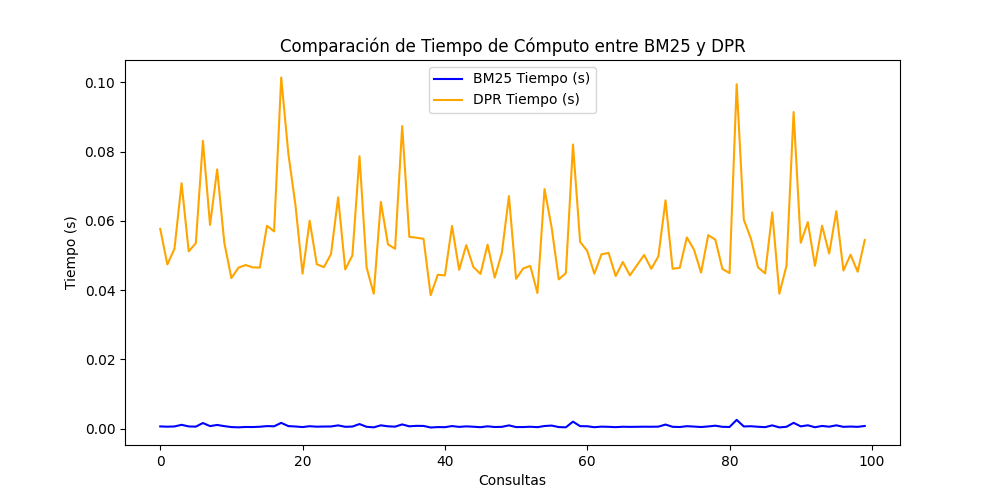
\includegraphics[width=0.7\textwidth]
    {img/tiempo_computo_comparacion.png}
    \caption{Uso de CPU}
    \label{fig:bm25_cpu_memory}
\end{figure}

\begin{figure}[h!]
    \centering
    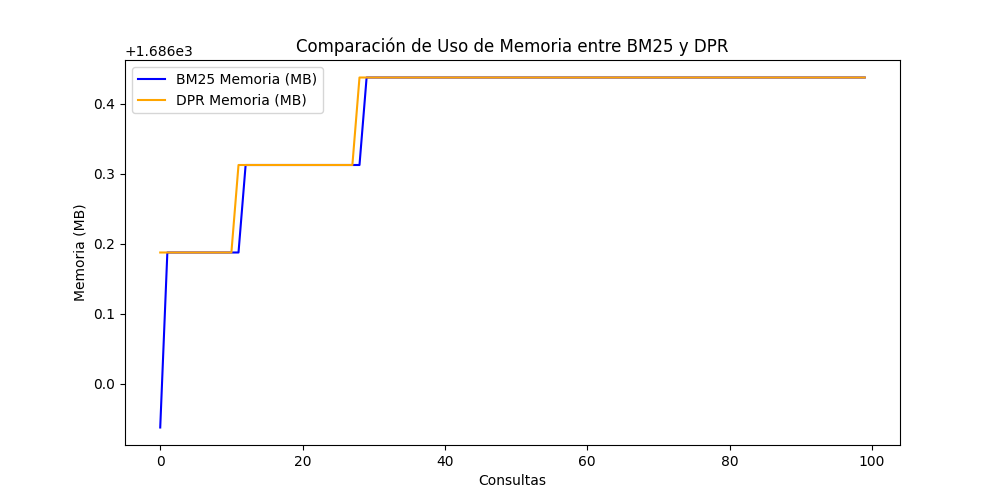
\includegraphics[width=0.7\textwidth]{img/uso_memoria_comparacion.png}
    \caption{Uso de memoria}
    \label{fig:dpr_cpu_memory}
\end{figure}

\section{Bibliografía}
\begin{thebibliography}{8}
\bibitem{bm25}
Robertson, S., Zaragoza, H.: The Probabilistic Relevance Framework: BM25 and Beyond. \emph{Foundations and Trends in Information Retrieval}, \textbf{3}(4), 333--389 (2009).

\bibitem{dpr}
Karpukhin, V., Oguz, B., Min, S., Lewis, P., Wu, L., Edunov, S., et al.: Dense Passage Retrieval for Open-Domain Question Answering. In \emph{Proceedings of the 2020 Conference on Empirical Methods in Natural Language Processing (EMNLP)}, 6769--6781 (2020).

\bibitem{transformers}
Wolf, T., Debut, L., Sanh, V., Chaumond, J., Delangue, C., Moi, A., et al.: Transformers: State-of-the-Art Natural Language Processing. \emph{Proceedings of the 2020 Conference on Empirical Methods in Natural Language Processing: System Demonstrations}, 38--45 (2020).

\end{thebibliography}

\end{document}

